\chapter{DroidWatcher}
\label{chap:droidwatcher}

\section{Presentation}
\label{sec:dw-presentation}

DroidWatcher is an application developed for the purpose of the current thesis.
It aims at demonstrating the concrete accessibility of localisation services.
By exploiting the official capabilities\footnote{A known bug has however been exploited for the remote GPS activation feature as explained in Section \ref{sec:dw-gps-bug}} of the Android operating system, a system actively monitoring the device movement has been developed.
For the purpose of this thesis the application takes only acceptable actions for the respect of user privacy.
But of course more invasive actions could be taken by malicious developers.

\begin{figure}[h]
  \centering
  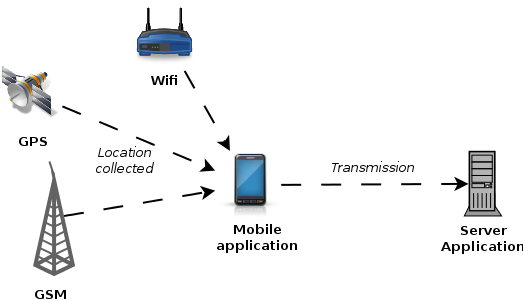
\includegraphics[width=9cm]{images/dw-archi.png}
  \caption{DroidWatcher system architecture}
  \label{fig:dw-archi}
\end{figure}

DroidWatcher is made of two major components as represented in Figure \ref{fig:dw-archi}: 

\begin{itemizealt}
\item A mobile application running on a smartphone:\\
  the application essentially collects location data on a regular basis.
\item A server-based application:\\
  the application centralises the data collected by the smartphones as soon as these smartphones have an Internet access.
\end{itemizealt}

In this chapter a detailed overview of the mobile application is given.
Installation guide and user manual on the complete DroidWatcher solution, on the mobile and server side, can be found in Appendix \ref{dw-guide}
% \section{Presentation}

% % In Chapter \ref{chap:and-loc}, it has been explained how the localization works in the Android devices.
% % What are the methods and how work the localization using wireless.
% % In Chapter \ref{chap:and-secu}, it has been explained how an application could behave through the Android system.
% % What is the control of the user, what are the limits of the permission system and how malwares abuse from the user confidence.\\

% DroidWatcher is an application that requests several permissions including the one to access the user location.
% Using this permission, the application can record the user permission at all time and monitor its movements.
% The application can be also controlled via text messaging invisibly and sends the recorded location over the Internet to a remote server.
% The application purpose is not to create a malware tracing devices but making the users realising what a device is capable of and how important it is to estimate the risk of malicious behaviour before installing an application.
% Also having having this application installed could be useful in case of loss or theft of the device.\\

% Appendix \ref{sec:dw-user-manual} contains the user manual and Appendix \ref{sec:dw-django} describe how to install the remote server application.

\section{Mobile application execution}

\subsection{Application structure}
\label{sec:dw-app-structure}

\begin{figure}[h]
  \centering
  \includegraphics[width=\textwidth]{images/dw-schema2.png}
  \caption{DroidWatcher execution process}
  \label{fig:dw-schema}
\end{figure}

Figure \ref{fig:dw-schema} shows the execution of the mobile application.
The application starts at phone boot, when unlocked or when the interface is used\footnote{Except with Android 4.0 or above where the interface should be launched at least once, see Section \ref{sec:dw-ics} for technical information}.
When starting, the application launch two  main components:

\begin{itemizealt}
\item Periodic actions
\item Event listener
\end{itemizealt}

Every specified amount of time (15~min by default), the current location and surroundings cell towers information (identifier and power strength) are recorded.
Is also verified if the phone is connected to the Internet to execute the online actions (upload of collected location and past cell phone towers localisation, see Section \ref{sec:dw-internet-actions}).\\

The event listener reacts to two types of event.
In the case of an SMS received, it proceeds to the adequate action (see Section \ref{sec:dw-sms-manag}).
The second watched event is the enabling of the wireless option on the mobile phone.
This event will test if an internet connection is successfully established and execute the online action in case of success.

\subsection{Location recording}

At the installation, the mobile application requests the localisation permissions\footnote{See Section \ref{sec:permissions} for details about the permission model}.
Using these permissions, every specified time interval (15~min by default), DroidWatcher records the location of the device.
The application works in background and keeps recording locations when the user does not use the smartphone.
Only the most accurate location is kept in an interval of 15~min.
Both GPS and network\footnote{The network resource is defined as the use of wireless and cell tower access points as described in Section \ref{sec:andro-wifi} and \ref{sec:loc-cell-tower}} resources are monitored using the officialy provided methods in Android.
If a new location is not available (the system keeps in cache the last recorded location), it will be ignored.
%Depending on what is available, it can use the GPS, wireless or GSM cell location capabilities, keeping the most accurate one.
The locations received are stored in a file on the SD card.\\

The surrounding cell data are also collected for future location.
The cell towers identifiers and signal strengths are recorded at the same frequency as the GPS and network locations.
The geographical coordinates of the collected GSM cell towers are retrieved once the phone is connected to the Internet and computed afterwards by using triangulation.

\subsection{Internet actions}
\label{sec:dw-internet-actions}

Periodically and when the wireless is enabled on the smartphone, the application verifies if the device is connected to the Internet.
When it is the case, the application takes two actions:

\begin{itemizealt}
\item Retrieving the geographical coordinates of the collected GSM cell towers and computing the previous locations using triangulation
\item Synchronising the collected locations to the remote server
\end{itemizealt}

The coordinates of the GSM towers are collected using an unofficial Google database available at \url{http://www.google.com/glm/mmap}.
This database has been selected as it is one of the most complete compared to the other free alternatives.
However, due to its unofficial state, it is possible the data will not be available in the future.\\

Using the geographical coordinates of the cell towers, the application is able to compute by triangulation of the previous location of the device.
The method developed to triangulate a device is explained in Section \ref{sec:dw-cell-triangu}.

\subsection{SMS management}
\label{sec:dw-sms-manag}

The mobile application provides a SMS-based command interface.
These commands allow configuration of the application (frequency of retrieval, server url, etc.) and take direct actions related to the location (enable GPS, return current location, etc.).
The application intercepts the received SMS before the main SMS application\footnote{The application is set to use the maximal priority in the chain of events. However, if another application has also set the maximal priority, it may retrieve the SMS before the DroidWatcher application.}.
If a predefined code is detected, it will discard the text message and will take an action accordingly.
Otherwise, the SMS is ignored and will be delivered to the main SMS application.\\

The complete list of SMS commands is available at Appendix \ref{sec:dw-smscom}.

\subsection{GPS activation}
\label{sec:dw-gps-bug}

The GPS of a device can be remotely activated using SMS command.
This feature is possible due to a bug discovered in the power control widget\footnote{Issue 7890 \url{https://code.google.com/p/android/issues/detail?id=7890}}.
Even if the security flaw has been revealed in April 2010 and a patch released in April 2011, the flaw has been observed as still exploitable on devices running Android 2.3.\\

This is the only part of the software where a bug is exploited in this application instead of using the official systems capabilities.
However, it is important for a user to understand that such flaws exist and, even when corrected, can affect a large part of devices (in August 2012, Android 2.3 and below represented 81\% of the Android market share).

%\emph{TODO: tester sur un Android 4.0}

\section{Cell tower triangulation}

\label{sec:dw-cell-triangu}



When a device needs to record the current location but is not capable to access the Internet, the program records the surrounding cell towers information.
The described triangulation algorithm is applied once the coordinates of the collected cell towers are retrieved, the next time the smartphone is connected to the Internet.

\subsection{Scenarios}

To triangulate a device using the cell towers, the following scenarios have been considered:

\begin{enumerate}
\item One GSM tower is within range
\item Two GSM towers are within range
\item More than two GSM towers are within range
\end{enumerate}

The case where no GSM towers are within range is not considered as the location can not be estimated and the algorithm is not used.
To evaluate the location, a \emph{centre point} is decided and a \emph{confidence range} is computed.
The device is estimated to be located within the area covered by the circle drawn using the centre point and the confidence as radius.\\

It has been decided not to differentiate the eventuality of more than three different cell towers as it will greatly increase the complexity of the algorithm without increasing the accuracy of the method proportionally, as intended by the limitations explained in Section \ref{sec:dw-difficult-cell}.

\subsection{Determine the position}

Depending of these three scenarios, the respective centres will be decided as:

\begin{enumerate}
\item The location of the only GSM tower within range
\item Along the median between the two GSM towers
\item \emph{The intersection between the two closest towers that is on the side of the third closest tower} Reformer
\end{enumerate}

If more than three GSM towers are within range, the closest towers are determined as the ones with the strongest signal strength.\\

\begin{figure}[h]
  \centering
  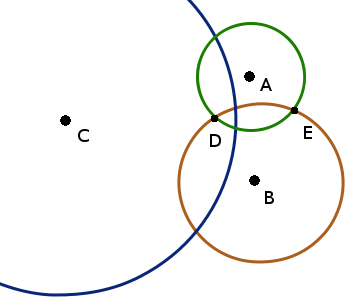
\includegraphics[width=8cm]{images/tower-schema.png}
  \caption{Triangulation scenario with 3 GSM towers}
  \label{fig:triangulation-scenario-3}
\end{figure}
The third scenario is illustrated in Figure \ref{fig:triangulation-scenario-3}.
The tower A and B are considered to be the closest to the device as received with the highest signal strength, the tower C is the third closest to the phone.
For each tower, a circle of a radius size related to the signal strength is drawn.
Two points D and E are computed as the intersection between the circles of centre A and B.
The point D is determined as the best centre point as it is the one closest to the tower C and is then evaluated as the location of the device.\\

In the three considered cases, the confidence range is determined as
\begin{enumerate}
\item The conversion of the signal strength to metres
\item The distance between the two intersections
\item The half of the distance between the two intersections
\end{enumerate}

%TODO \emph{Comment justifier l'utilisation de la distance ?}

\subsection{Signal strength conversion}

If a device receives a GSM signal at a determined strength, it is possible to estimate its distance from the cell tower.
A circle is drawn around the GSM tower representing every position the device could take.
The stronger the signal is, the closer the device is to the tower.\\

The signal strength collected by the Android device is expressed in \emph{ASU}, for Arbitrary Strength Unit, which is a value between 0 and 31 derived from the signal strength usually computed in decibels\footnote{For the GSM network, $dBm = 2 * ASU - 113$}.
0 ASU representing the lowest signal and 31 the strongest.
The conversion is expressed by the following formula :\\

\[
 (-\sqrt{asu}+6)*900
\]

The weighting of the factors has been decided based on personal observations using the author's smartphone.
Successive locations were recorded and compared to the location of the cell tower and signal strenght.

\section{Technical challenges}

To develop this application, several constraints were experienced that limited the effect of the application.

\subsection{Automatic idle}

Once going in idle state (once the device is not used by the user for a certain amount of time), the operating system will limit the possibility of the system to save battery.
Some applications will be paused during its running process.
The effectiveness of the localisation process done by DroidWatcher is affected by this idle purpose.\\

This is the case, for example, of the GPS that needs to constantly update the position.
The GPS may sometimes stop monitoring the position of the user if it can not get a fix\footnote{See Section \ref{sec:loc-gps} for the information needed to get a GPS fix} on the location of the user.
This effect is independent from the application but is the direct consequence of battery saving measures taken by the system. 
This issue is often a complaint related to the tracking application (eg: sport monitoring application).
A solution is stop the phone from going to idle state by keeping it in awake state.
However, this solution is not used in DroidWatcher as it would have greatly compromised the battery consumption  of the phone and consequently the effectiveness of the application in monitoring the location for an extended period of time and as discretely as possible.

\subsection{Android 4.0}
\label{sec:dw-ics}

The author of this thesis owns a device with Android 2.3 and this device was used in the process of the research. 
At the time of development, end of 2011, the fourth version of Android\footnote{The third version of the operating system was limited to tablet devices and not phones limiting greatly the propagation of this version of the system.} was just released and very few devices were capable of running it.
Consequently the testing has been done mainly on devices running the second version of the operating system.\\

An unexpected change introduced in the 4.0 version\footnote{The change was already present since the version 3.1 for tablets but reflected to smartphones only since the version 4.0} of Android is the way a device manages the start of an application in background.
DroidWatcher has been conceived to be started when a device is booting or waked from idle.
This feature supported the aim to be fully discrete and ensured that the application was not noticeable without analysis.
With Android 4.0, an application can no longer start during the boot or after having been woken up if the interface has not been launched first time~\cite{boot-restrictions}.\\

To fix this problem, an interface screen has been developed.
This screen allows the user to see location information and basic configuration.\\

This change is certainly an improvement in the security of a device as the need for a graphical interface will strongly reduce the possibility to run a malicious \emph{invisible} application.
However malicious applications often use a fake interface (weather forecast, game, etc.) to hide the malicious behaviour of the software and this protection will therefore not affect these applications.

\subsection{Cell tower triangulation}
\label{sec:dw-difficult-cell}

To compute the location of the user, a triangulation algorithm has been developed.
This algorithm is however known as imprecise for several reason.
A basic triangulation algorithm was used to compute circle intersections\footnote{Intersection of two circles by  Graeme McRae \url{http://2000clicks.com/mathhelp/GeometryConicSectionCircleIntersection.aspx}} but the unknown factor is the relation between the received signal strength and the distance from the cell tower.\\

To compute the location, the algorithm uses the signal strength of captured GSM cell towers nearby.
The signal strength is a very fluctuating variable.
At a same distance to a cell tower, the signal varies if the device is inside or outside a building or if monitored by two different devices with different GSM receiver.
The main imprecision comes from the fact that all cell tower do not emit signal at the same signal strength (rural areas are usually covered with less cell towers emitting using higher signal strengths.\\

As efficient computation of the signal strength would have required long monitoring and observation on a large number of devices and areas.
The computation and weighting of the variables has been done based on personal observations.
This is known as imprecise but achieves the purpose of being able to record a reasonable approximation of the location at any time when GSM connectivity is available.\\

